\documentclass{beamer}
%\beamerdefaultoverlayspecification{<+->}
\usepackage{soul}
\usepackage{listings}

\usetheme{Berlin}

\title{Aplicativo web de auxílio à navegação aérea}
\author{Antenor Barros Leal}
\institute{Departamento de Informática \\ PUC-Rio}
\date{Dezembro 2024}

\begin{document}

\begin{frame}
    \titlepage
\end{frame}

\begin{frame}{Outline}
    \tableofcontents
\end{frame}

\section{Introdução}

\begin{frame}{Introdução}
    \begin{figure}[ht]
        \begin{minipage}[b]{0.45\linewidth}
            \centering
            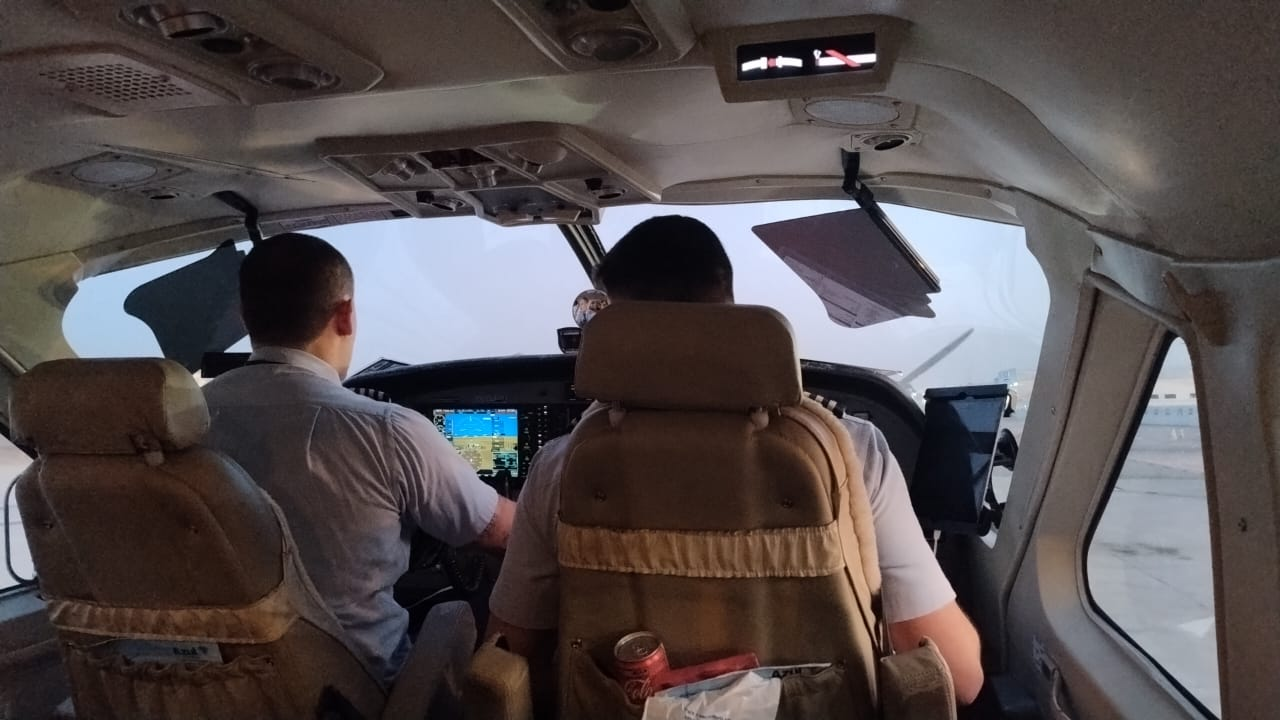
\includegraphics[width=\textwidth]{img/efb-real-original.jpg}
            \caption{Electronic Flight Bag (David Guimarães)}
        \end{minipage}
        \hspace{0.5cm}
        \pause
        \begin{minipage}[b]{0.45\linewidth}
            \centering
            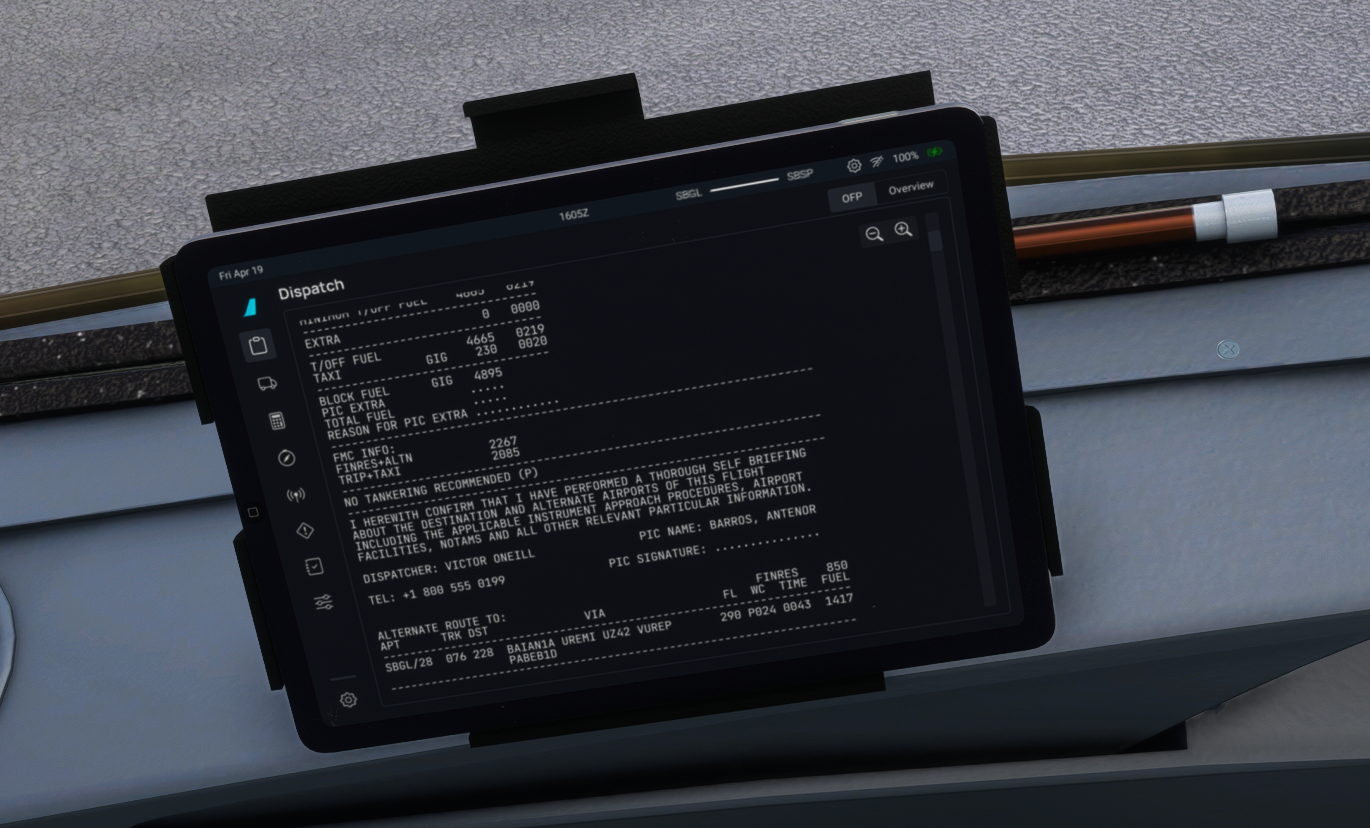
\includegraphics[width=\textwidth]{img/efb-a320.png}
            \caption{Electronic Flight Bag (MSFS2020 / FlyByWire Simulations)}
        \end{minipage}
    \end{figure}
\end{frame}

\begin{frame}{Introdução}
    \begin{itemize}
        \item Restrição para simulação de voo
    \end{itemize}
    \pause
    \begin{figure}[ht]
        \begin{minipage}[b]{0.45\linewidth}
            \centering
            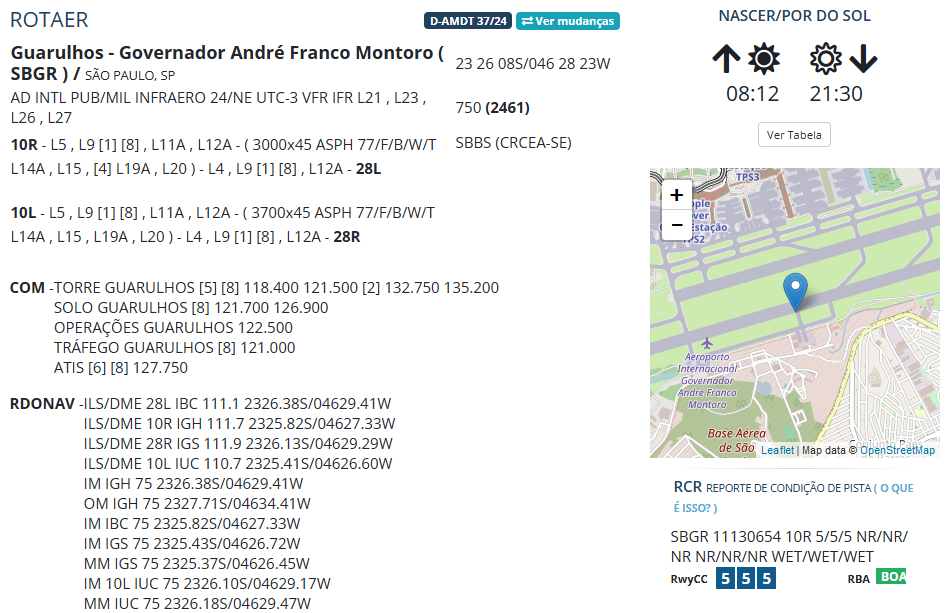
\includegraphics[width=\textwidth]{img/aisweb.png}
            \caption{AISWEB}
        \end{minipage}
        \hspace{0.5cm}
        \pause
        \begin{minipage}[b]{0.45\linewidth}
            \centering
            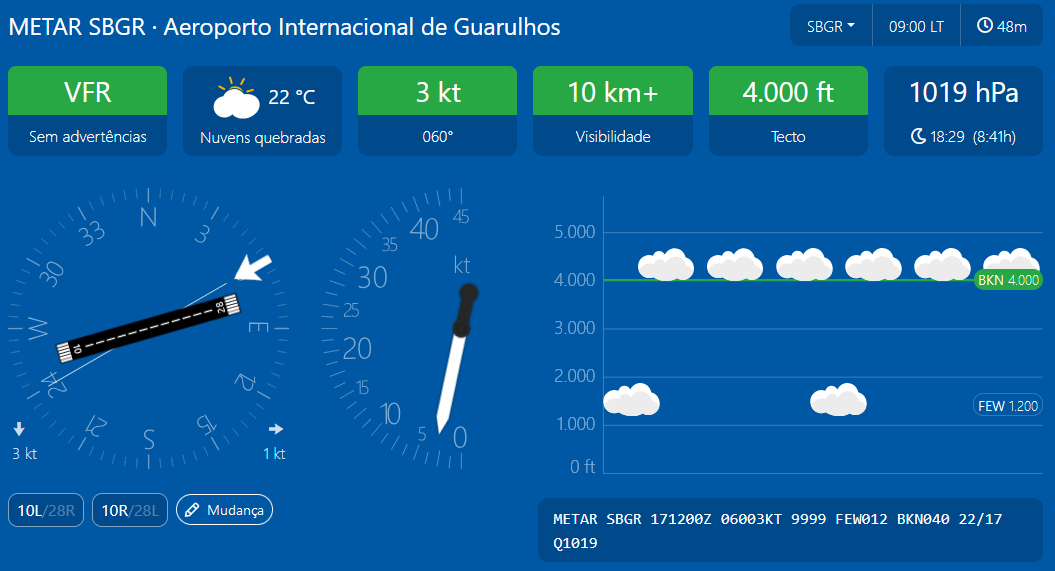
\includegraphics[width=\textwidth]{img/metar-taf.png}
            \caption{METAR-TAF}
        \end{minipage}
    \end{figure}
\end{frame}

\begin{frame}{UI}
    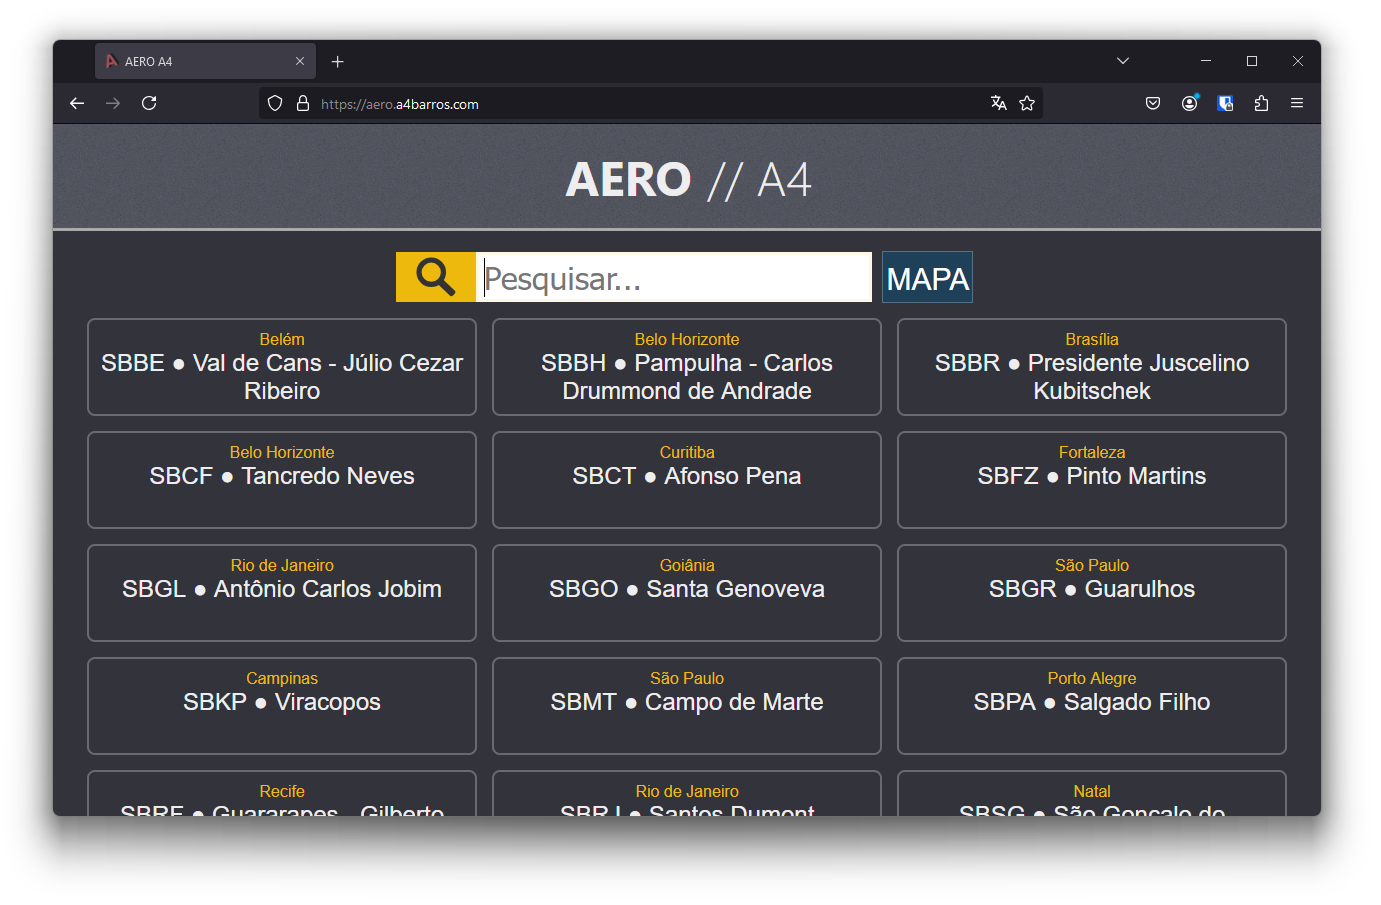
\includegraphics[width=0.7\linewidth]{img/UI.png}
    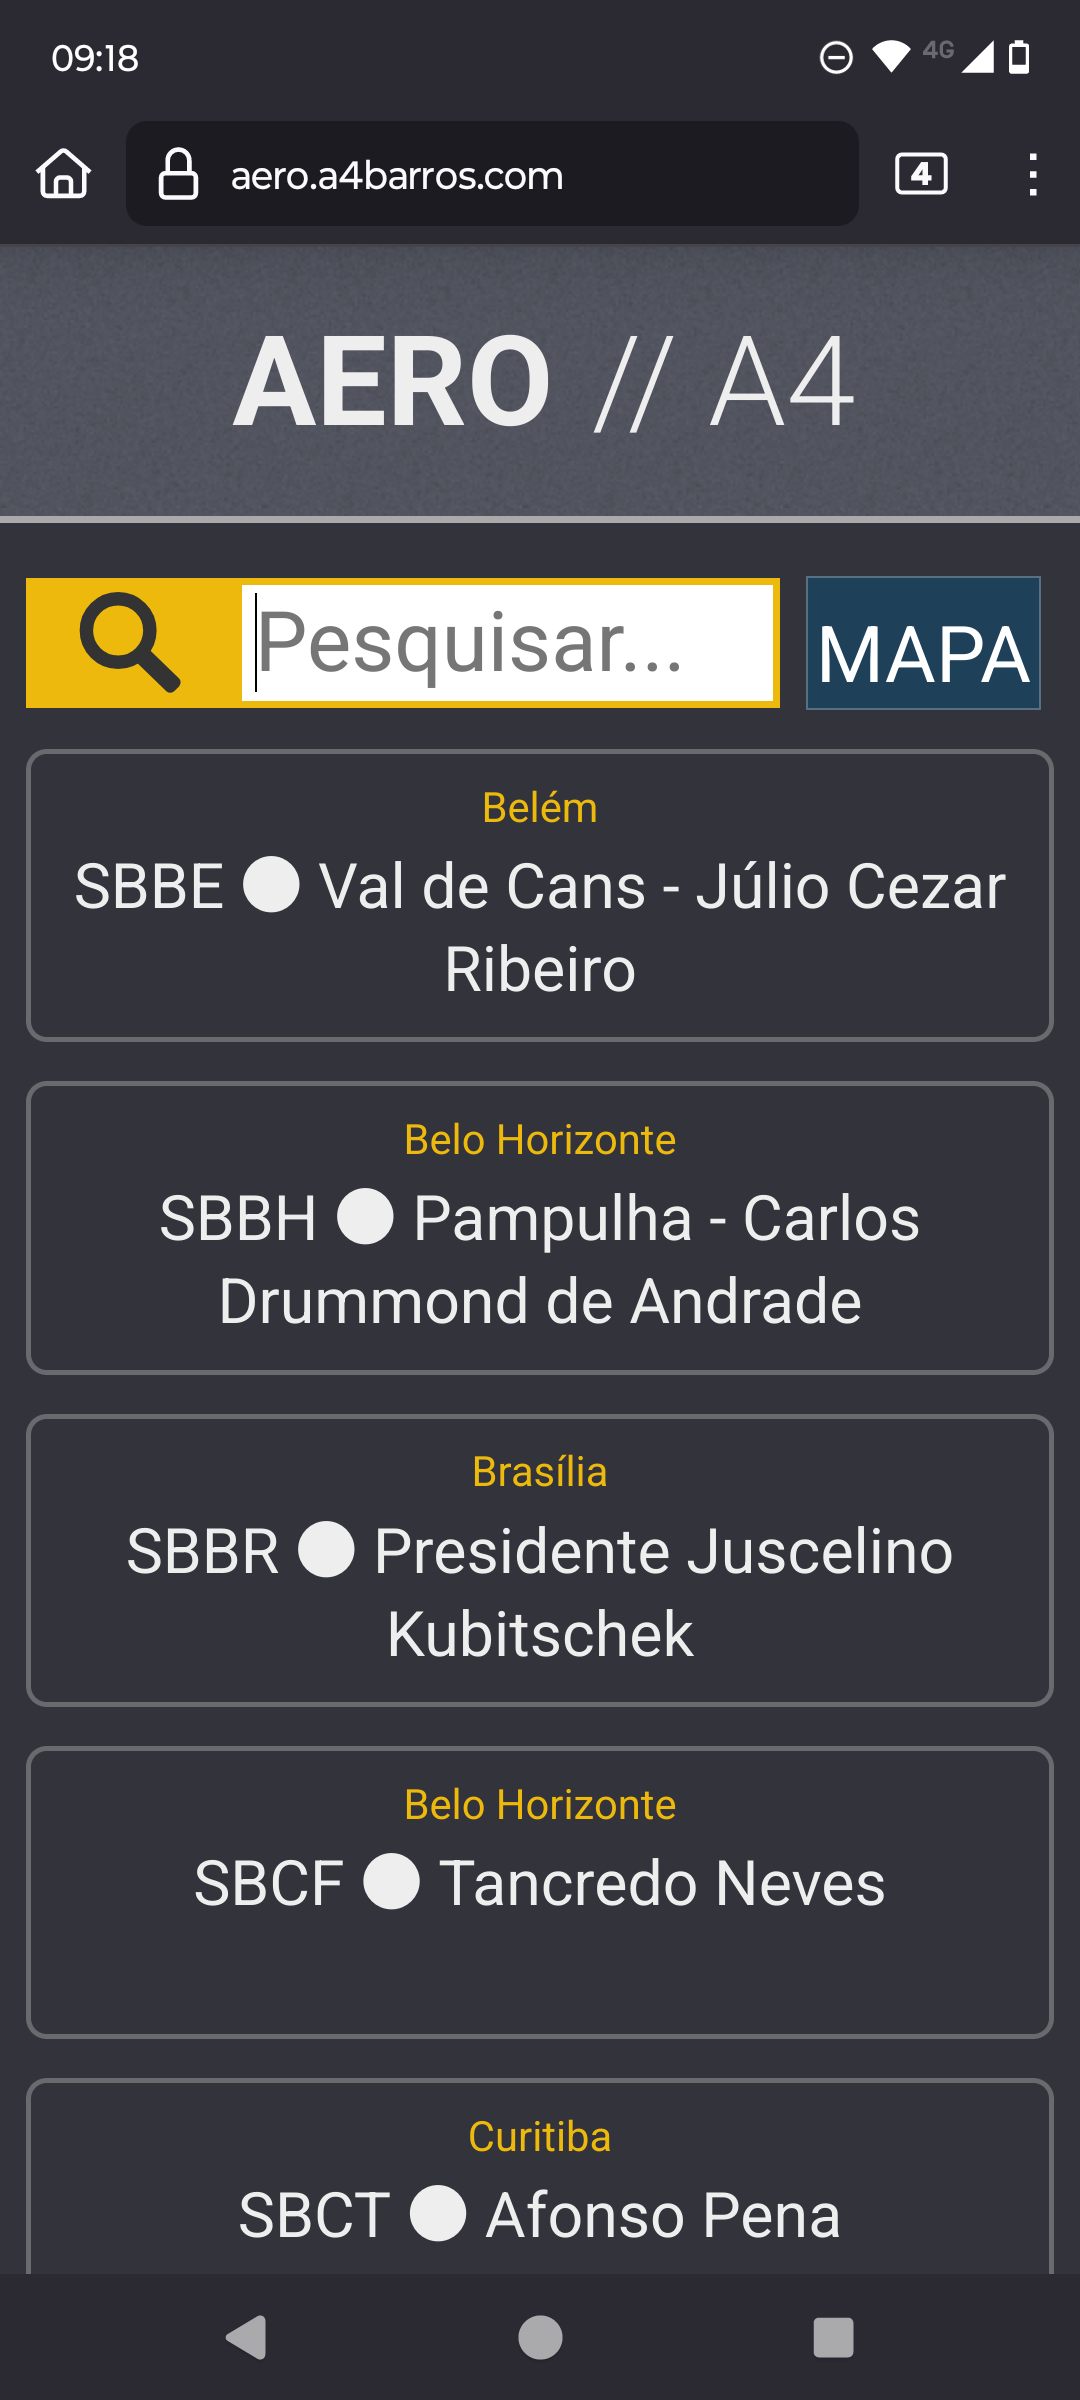
\includegraphics[width=0.2\linewidth]{img/UI_mobile.png}  
\end{frame}


\section{Arquitetura}

\begin{frame}{Servidor}
    \begin{figure}[ht]
        \begin{center}
        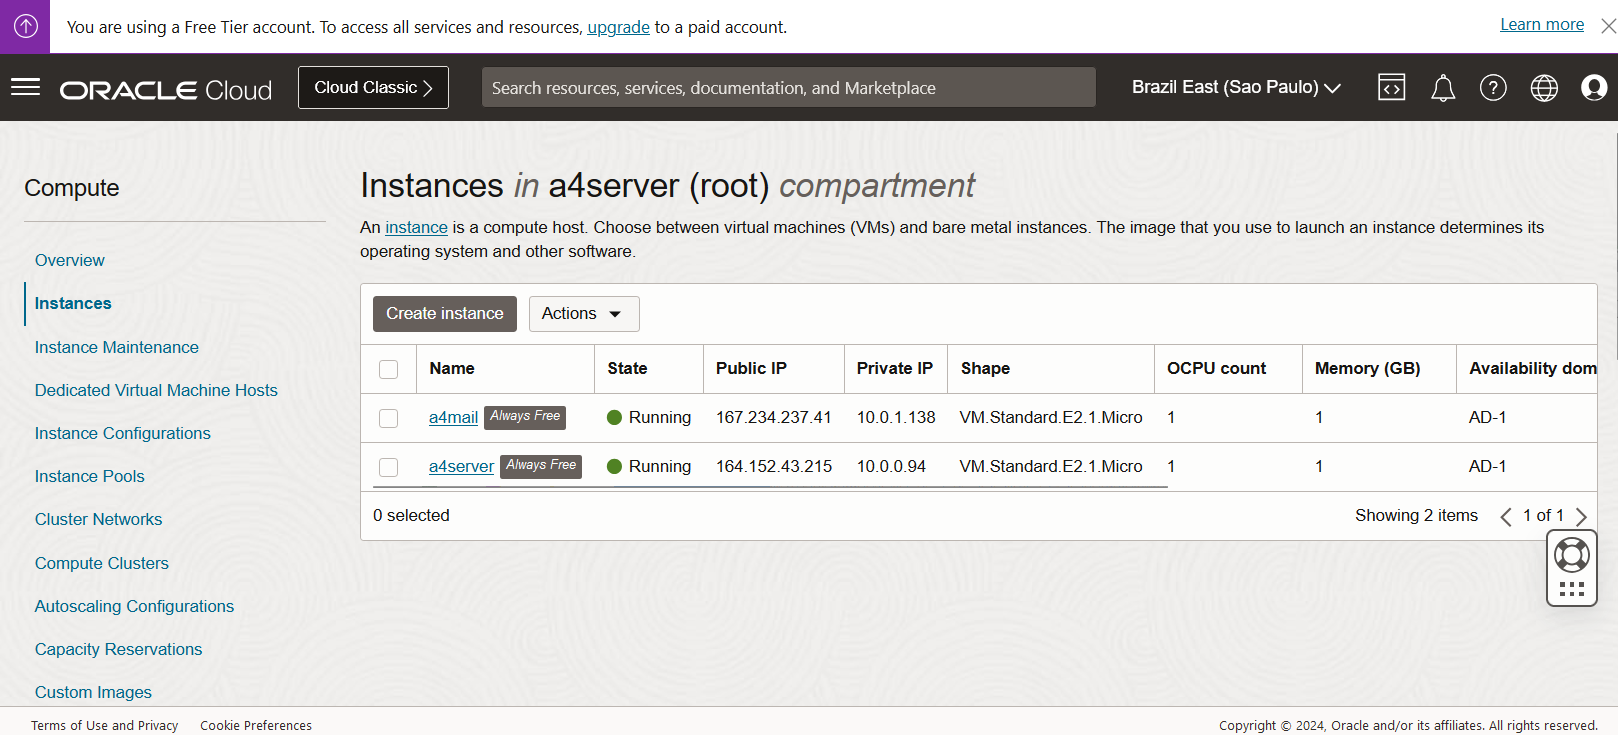
\includegraphics[width=0.6\linewidth]{img/oracle.png}
        \label{fig:UI}
        \end{center}
    \end{figure}
    \pause
    \begin{columns}
        \begin{column}{0.5\textwidth}
            \begin{itemize}
                \item \textbf{CPU:} AMD EPYC 7551 (2 cores) @ 1.996GHz
                \item \textbf{RAM:} 1GB
                \item \textbf{Armazenamento:} 25GB
                \item \textbf{SO:} Ubuntu 22.04 LTS
            \end{itemize}
        \end{column}
        \pause
        \begin{column}{0.5\textwidth}
            Upgrade
            \begin{itemize}
                \item \textbf{CPU:} Ampere Altra
                \item \textbf{RAM:} 8GB
                \item \textbf{Armazenamento:} 50GB
                \item \textbf{SO:} Ubuntu 22.04 LTS
            \end{itemize}
        \end{column}
    \end{columns}
\end{frame}

\begin{frame}{Arquitetura}
    \begin{itemize}
        \item \textbf{Infra:} Docker/Docker Compose
        \pause
        \item \textbf{Proxy reversa:} NGINX
        \pause
        \item \textbf{Banco:} MariaDB
        \pause
        \item \textbf{Backend:} \st{Flask} FastAPI
        \pause
        \item \textbf{Frontend:} Jinja2
        \pause
        \item \textbf{Observabilidade:} GoAccess
        \item Outros subdomínios
    \end{itemize}
\end{frame}

\begin{frame}{Diagrama da arquitetura}
    \begin{figure}[ht]
        \begin{center}
        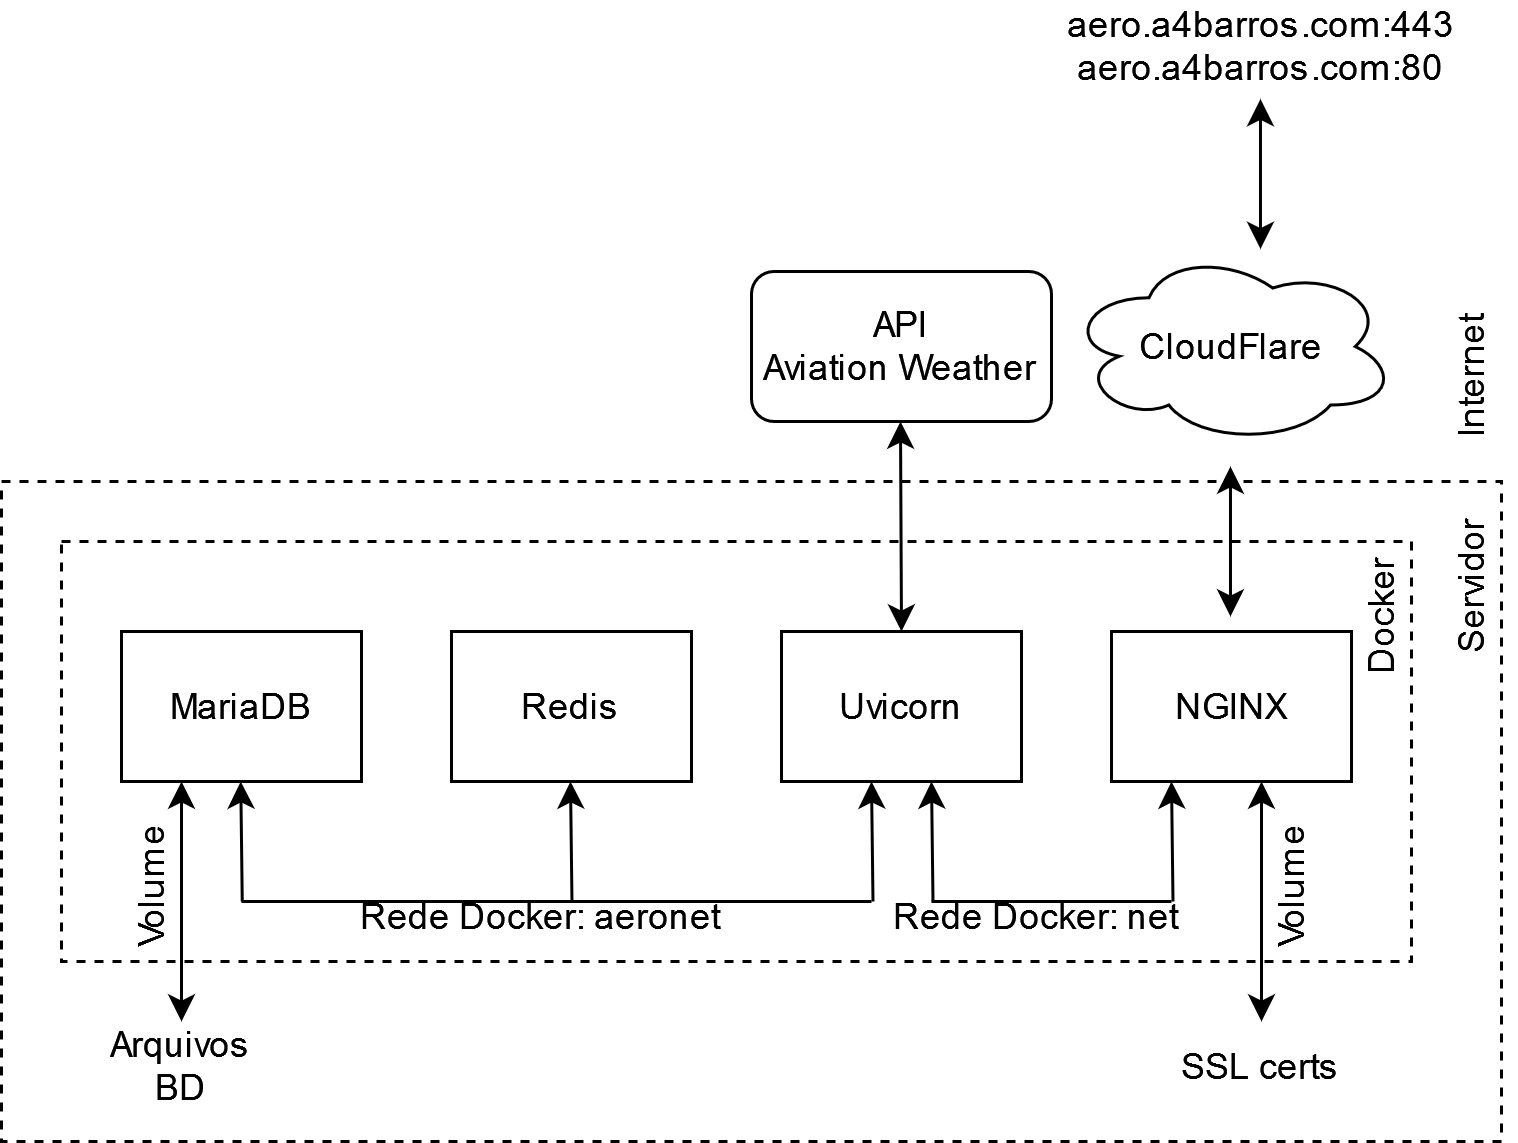
\includegraphics[width=0.65\linewidth]{img/arquitetura.png}
        \label{fig:arquitetura}
        \end{center}
    \end{figure}
    \begin{itemize}
        \item Uso de Docker network e volumes
    \end{itemize}
\end{frame}

\begin{frame}{Diagrama de tempo}
    \begin{columns}
        \begin{column}{0.5\textwidth}
            \begin{itemize}
                \item Tarefas \textbf{síncronas}
                    \begin{itemize}
                        \item Rotas
                    \end{itemize}
                \pause
                \item Tarefas \textbf{assíncronas}
                    \begin{itemize}
                        \item METAR (20 min)
                        \item TAF (4 h)
                        \item Plots (20 min)
                    \end{itemize}
            \end{itemize}
        \end{column}
        \pause
        \begin{column}{0.5\textwidth}
            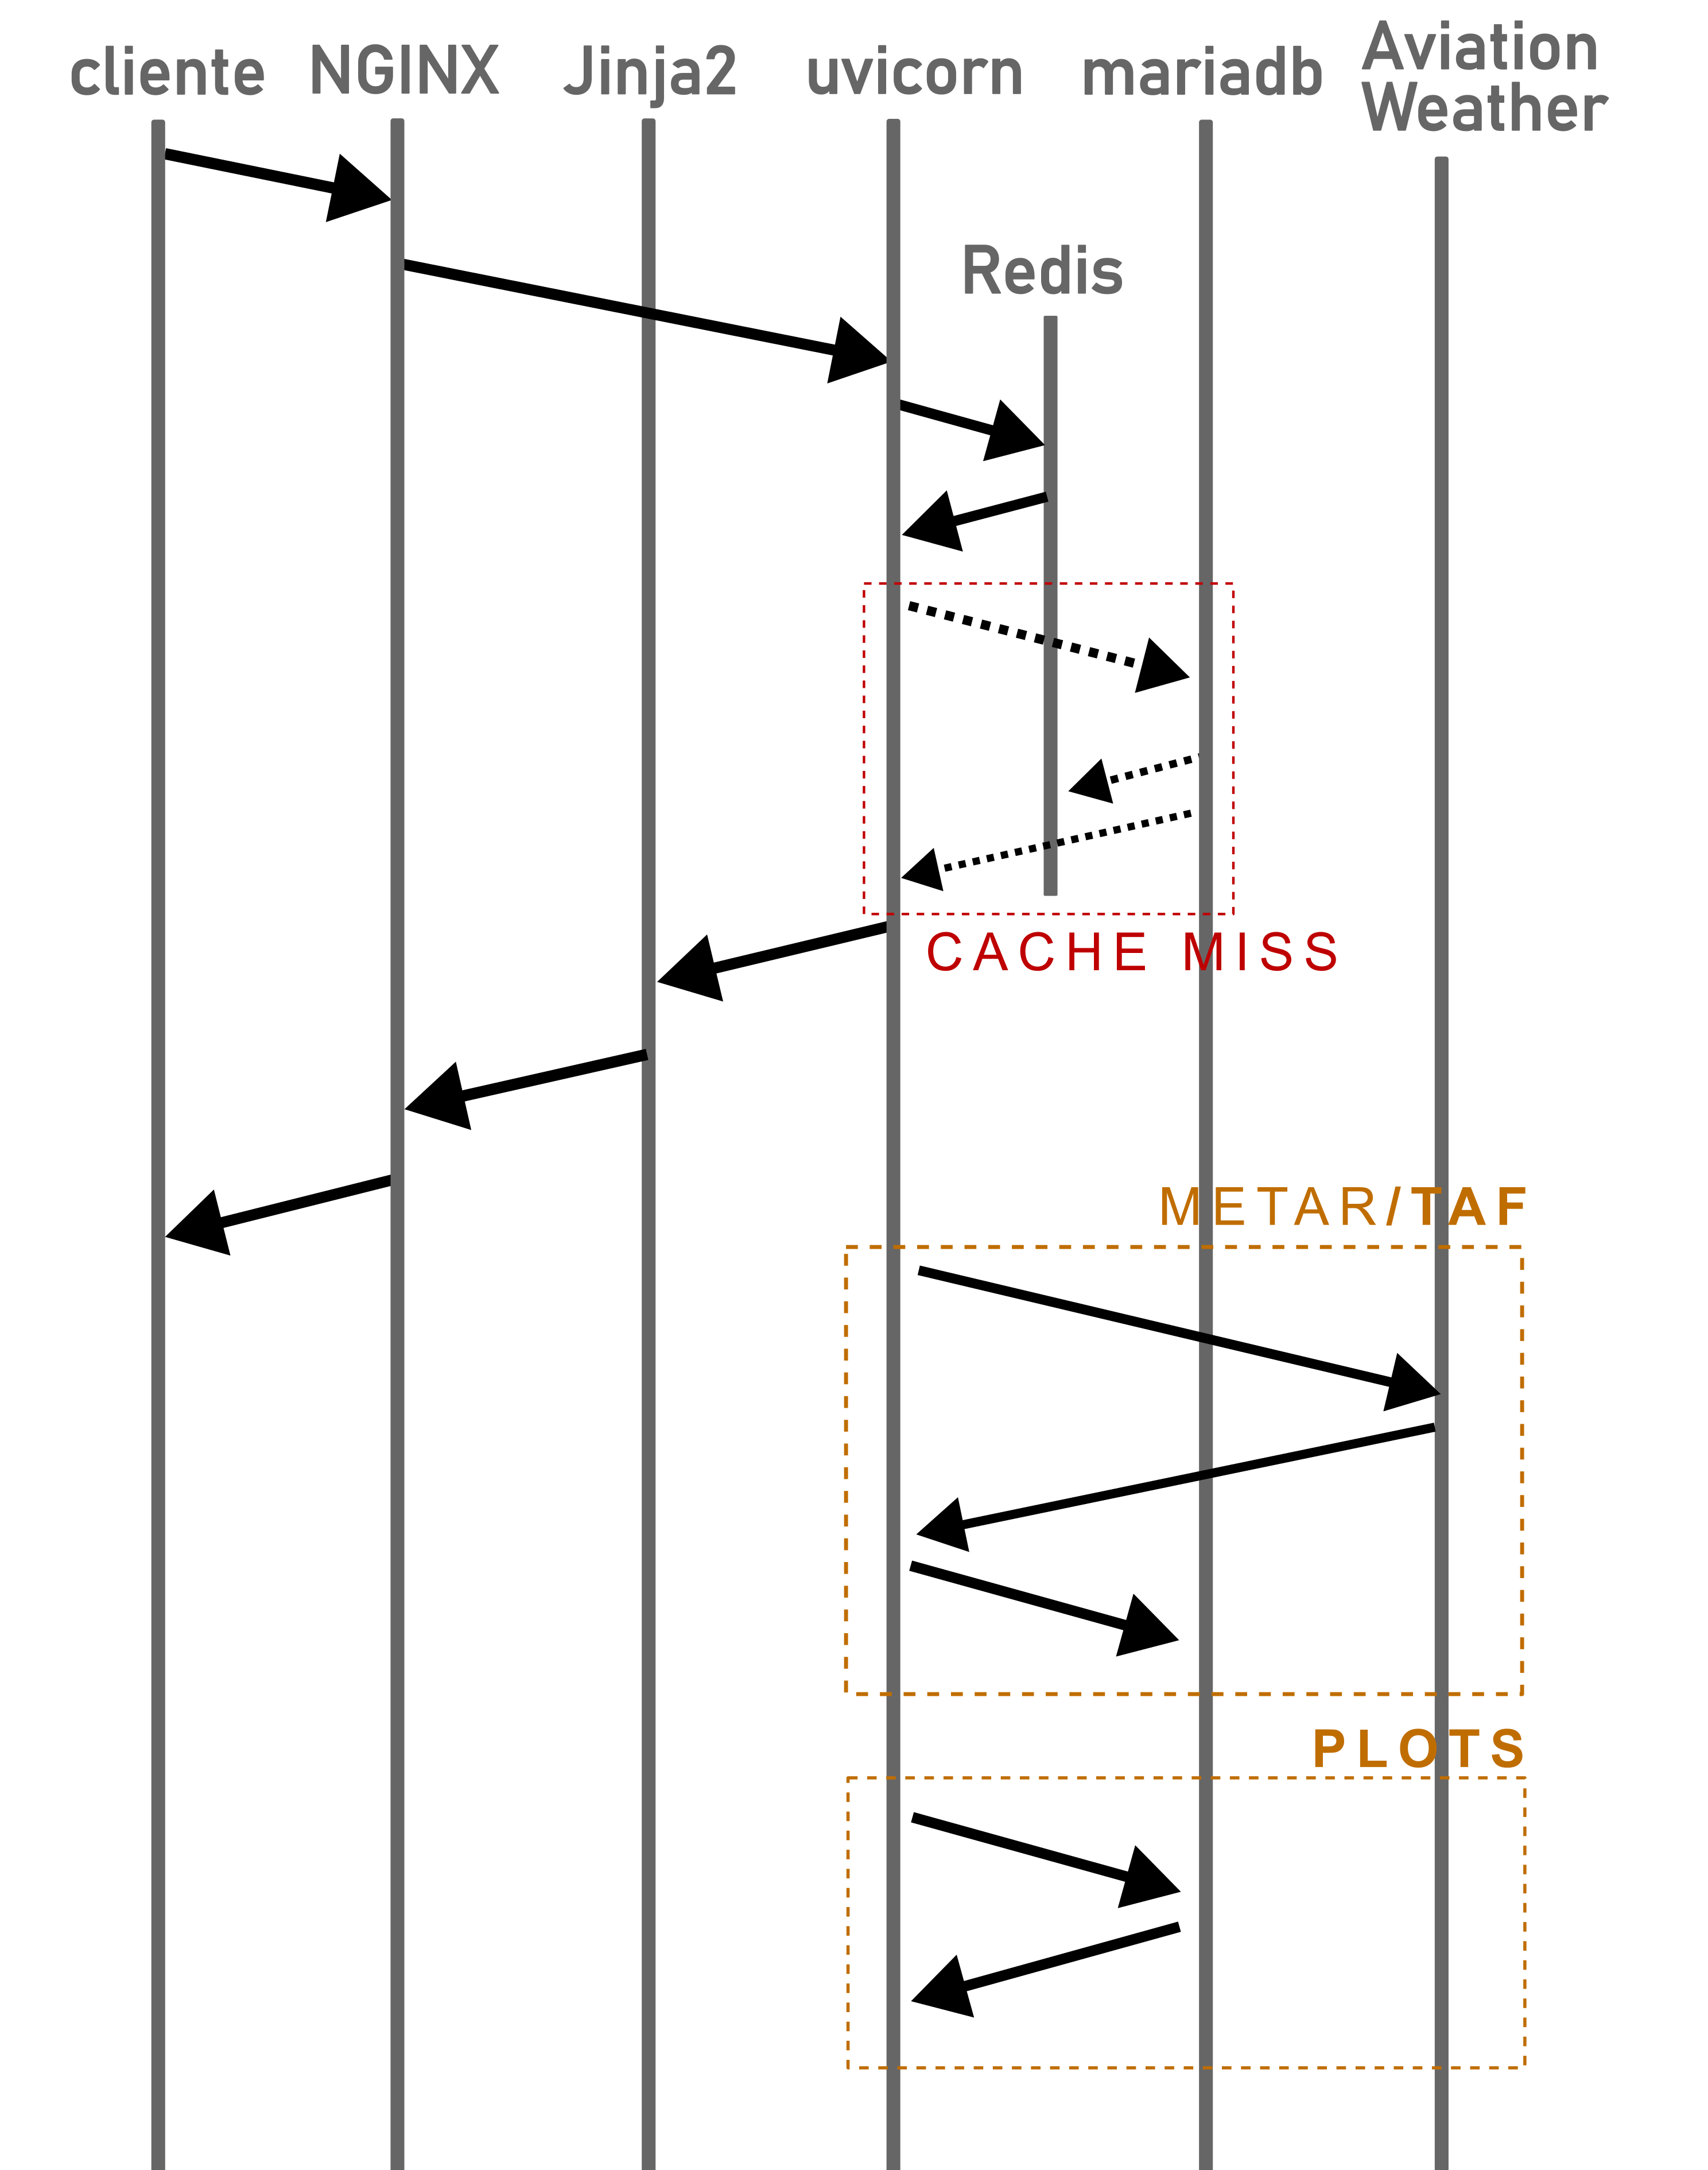
\includegraphics[width=0.9\linewidth]{img/diagrama-tempo.png}
        \end{column}
    \end{columns}
\end{frame}

\begin{frame}{Uso de rescursos}
    \begin{itemize}
        \item 500 acessos simultâneos (usando Locust)
    \end{itemize}
    \pause
    
    \begin{figure}[ht]
        \begin{center}
        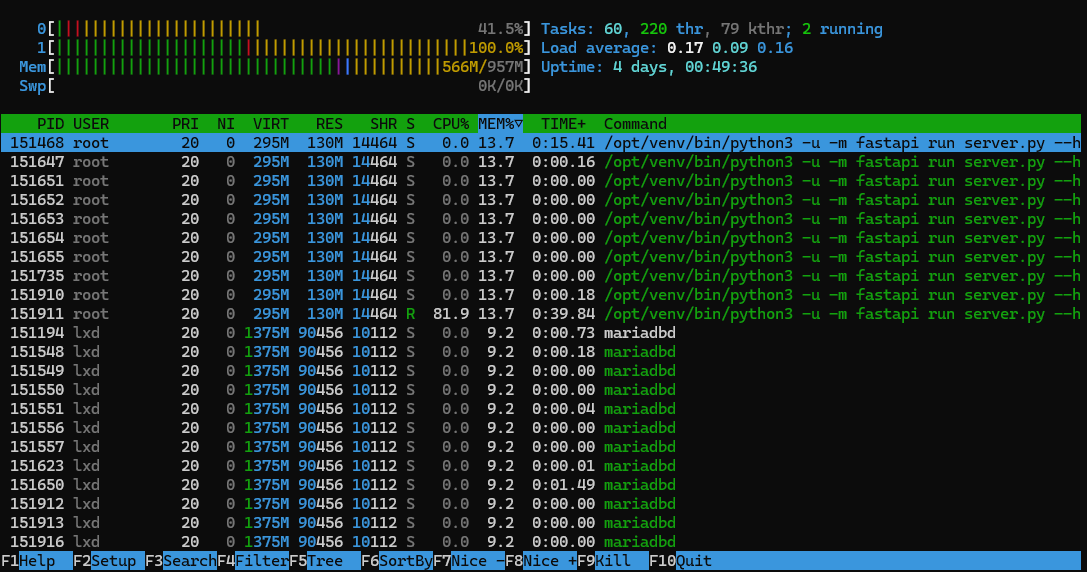
\includegraphics[width=0.8\linewidth]{img/server-500-acessos.png}
        \label{fig:arquitetura}
        \end{center}
    \end{figure}
\end{frame}


\section{Projeto}

\begin{frame}{Tabelas}
    \begin{figure}[ht]
        \begin{center}
        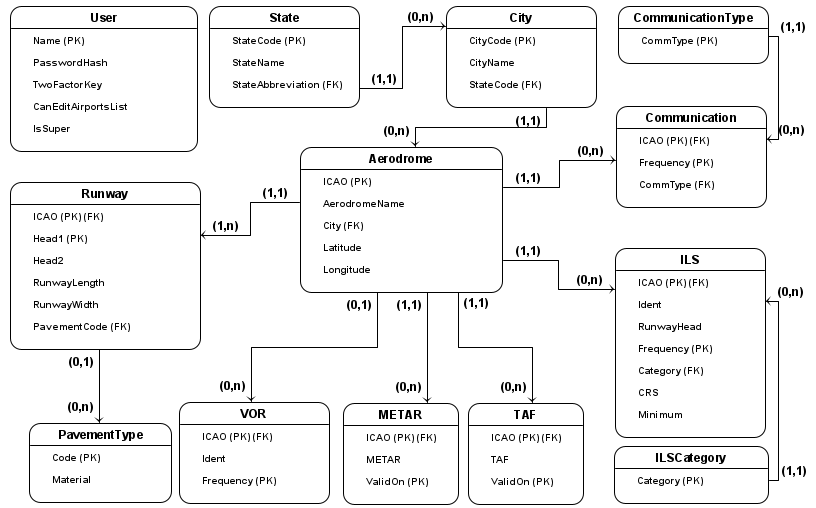
\includegraphics[width=0.8\linewidth]{img/ERAero.png}
        \label{fig:arquitetura}
        \end{center}
    \end{figure}
\end{frame}

\begin{frame}{METAR}
    \centering
    \begin{itemize}
        \item Separação nos espaços
        \item Regex
        \item Lista de tuplas
        \item Ferramenta de templating
    \end{itemize}

    \begin{minipage}[b]{0.9\linewidth}
        \begin{columns}
            \begin{column}{0.4\textwidth}
                \tiny{\texttt{251600Z 22011KT 9999 BKN023 OVC035 21/16 Q1012}}
            \end{column}
            \begin{column}{0.6\textwidth}
                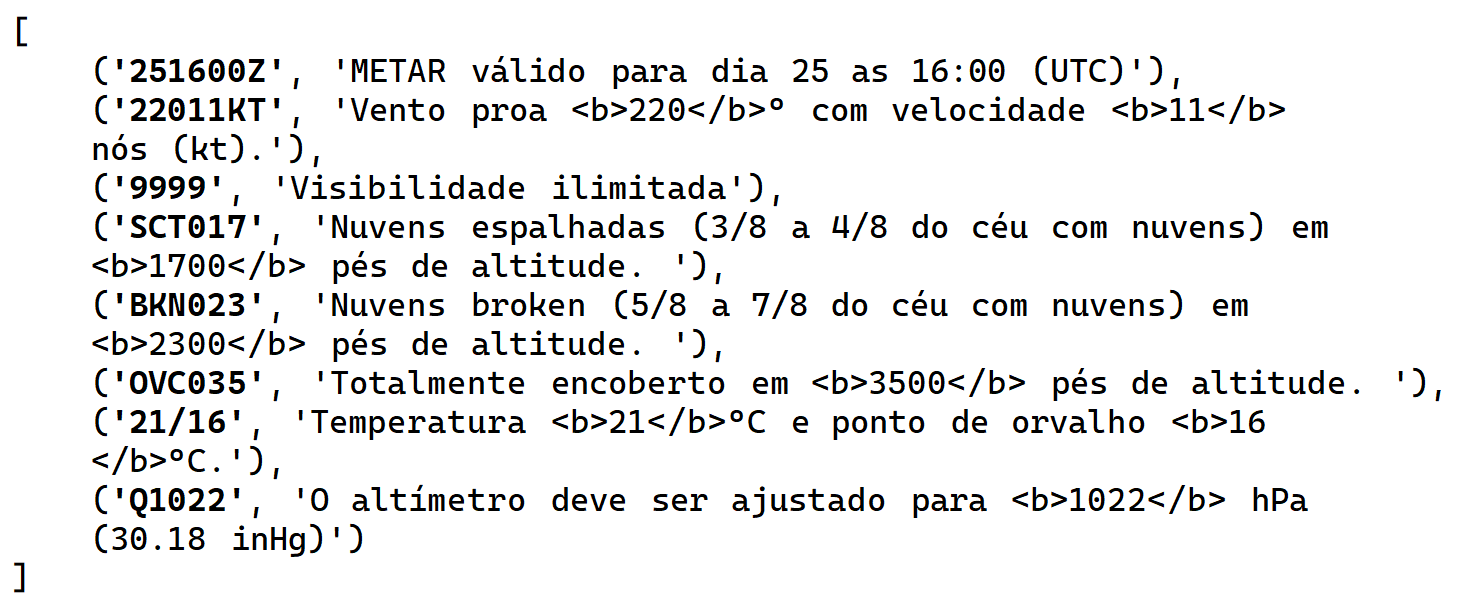
\includegraphics[width=\linewidth]{img/metar-dec.png}
            \end{column}
        \end{columns}
    \end{minipage}
\end{frame}

\begin{frame}{TAF}
    \footnotesize{\texttt{
220859Z 2212/2312 06006KT 9999 SCT040 TX34/2217Z TN24/2309Z \\
    BECMG 2215/2217 34013KT SCT040 FEW045TCU \\
    TEMPO 2220/2222 TS SCT030 FEW035CB \\
    BECMG 2222/2224 04008KT CAVOK \\
    BECMG 2310/2312 SCT020 RMK PGX}}

  \begin{figure}[ht]
    \begin{center}
    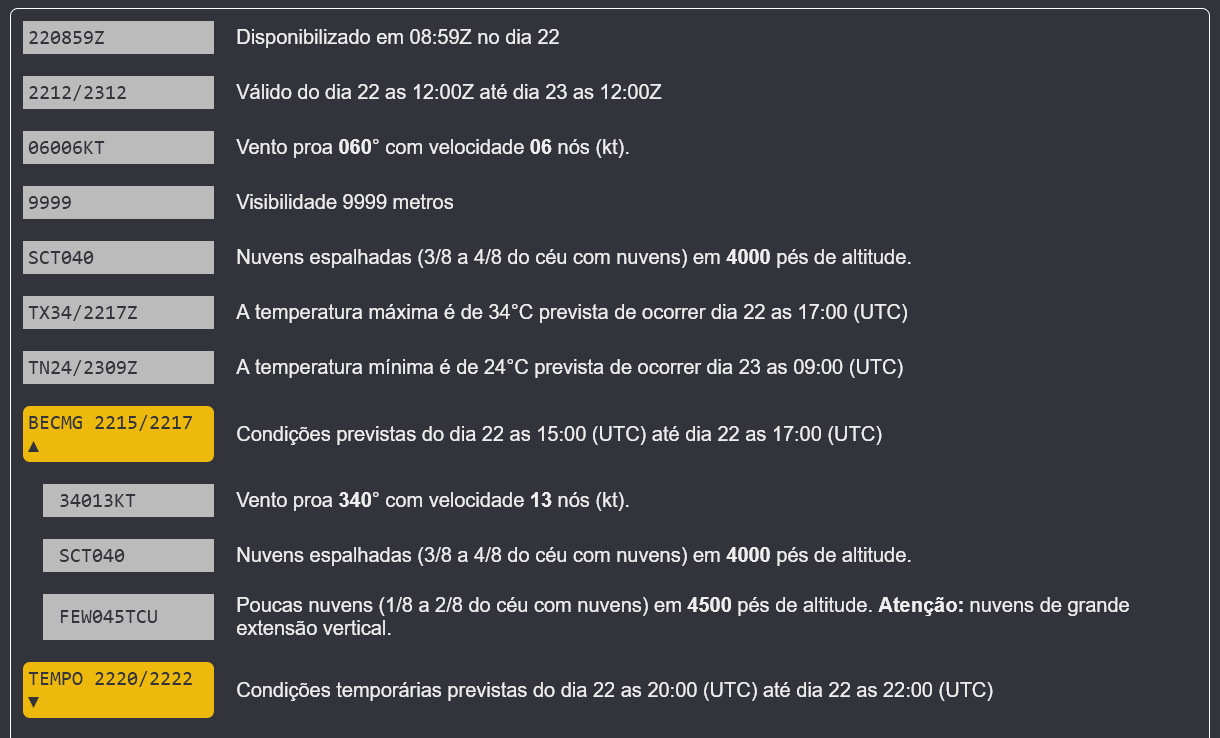
\includegraphics[width=0.65\linewidth]{img/TAF-SBBE.png}
    \label{fig:UI}
    \end{center}
    \end{figure}
\end{frame}

\begin{frame}{Histórico}
    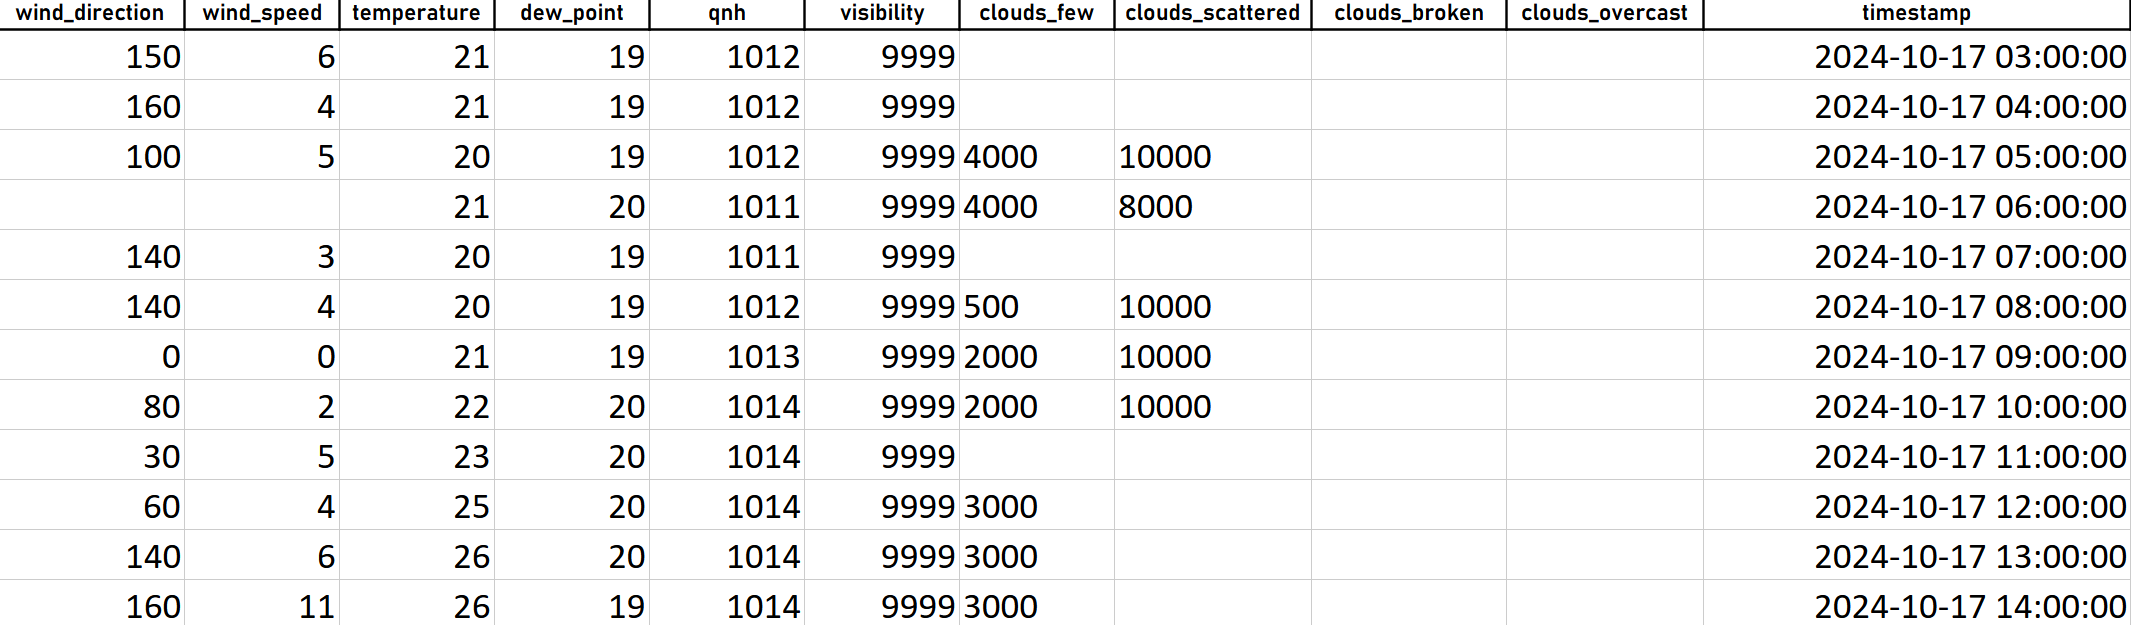
\includegraphics[width=0.9\linewidth]{img/image.png}
\end{frame}

\begin{frame}{Histórico}
    \begin{figure}[ht]
        \begin{center}
        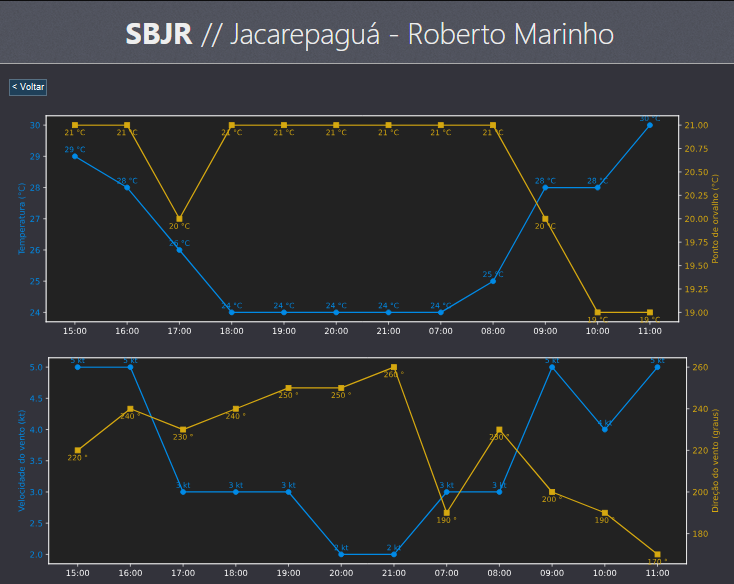
\includegraphics[width=0.7\linewidth]{img/history-1.png}
        \label{fig:UI}
        \end{center}
    \end{figure}
\end{frame}

\begin{frame}{Histórico}
    \begin{figure}[ht]
        \begin{center}
        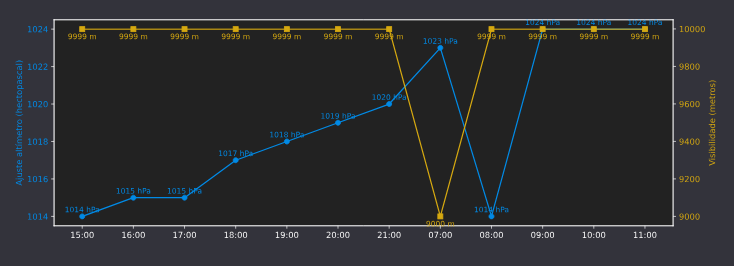
\includegraphics[width=0.7\linewidth]{img/history-2.png}
        \label{fig:UI}
        \end{center}
    \end{figure}
\end{frame}


\section{Teste de carga}

\begin{frame}{Sem cache}
    \begin{itemize}
        \item Modo desenvolvedor CloudFlare
    \end{itemize}    

    \begin{center}
        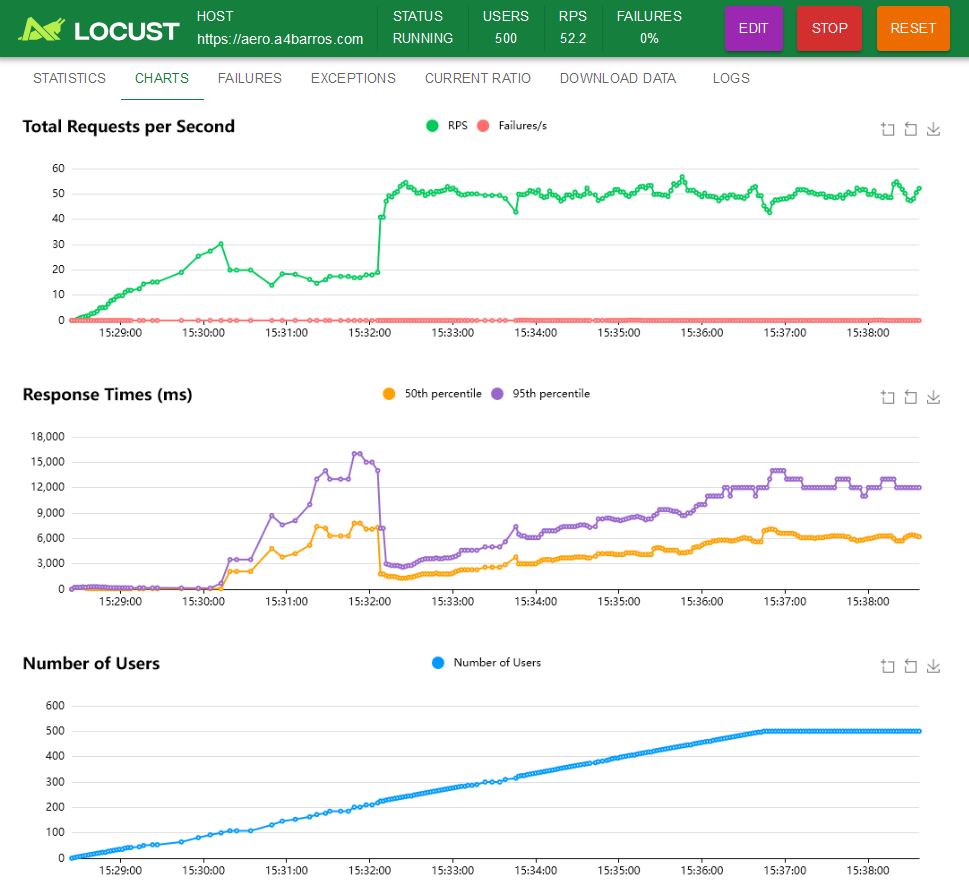
\includegraphics[width=0.6\linewidth]{img/locust-no-cache.png}
    \end{center}
\end{frame}

\begin{frame}{Cache Redis}
    \begin{itemize}
        \item Decorator implementado: \@cache\_it
    \end{itemize}

    \begin{center}
    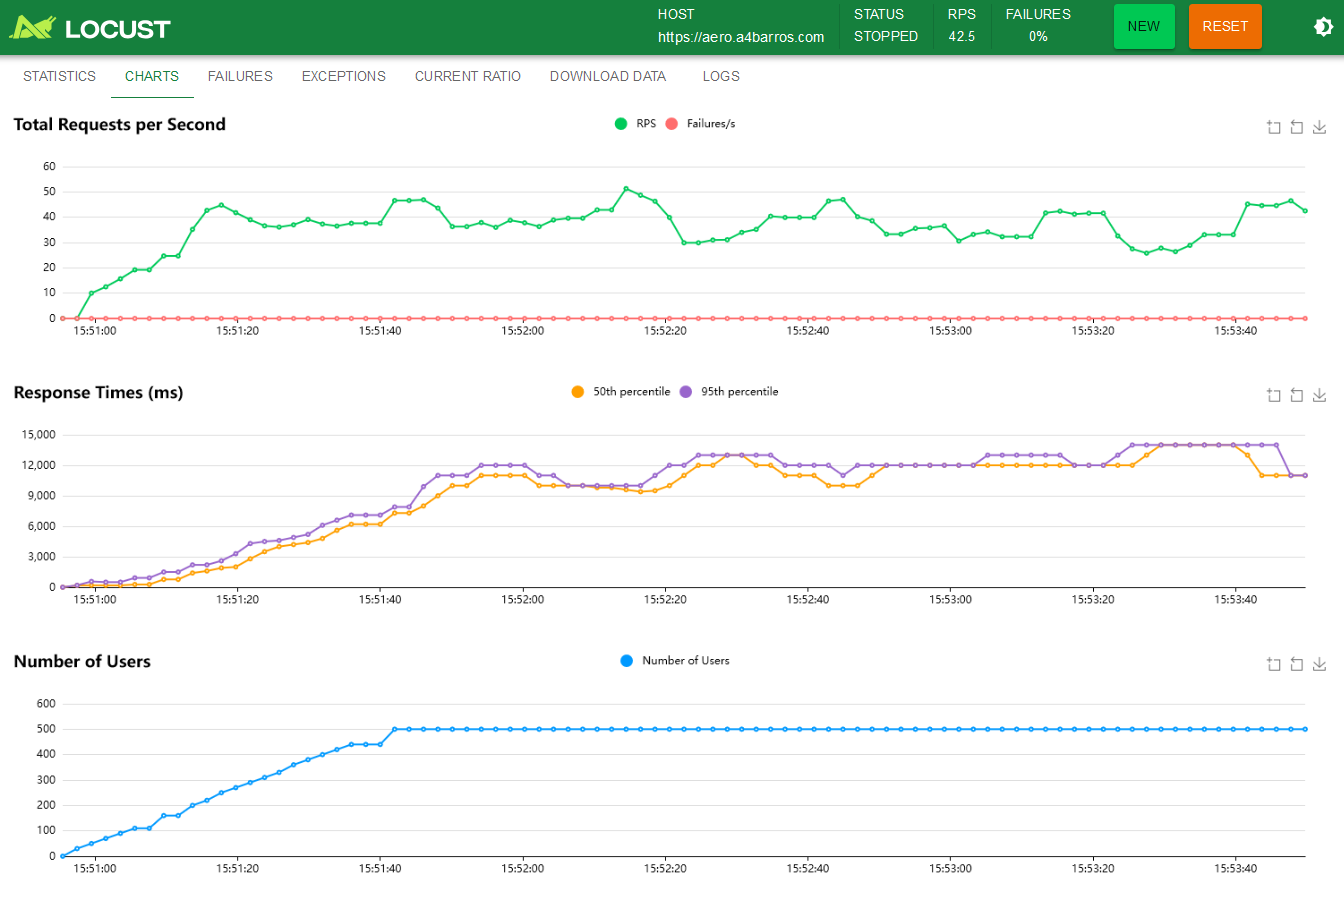
\includegraphics[width=0.6\linewidth]{img/locust-cache-redis.png}
    \end{center}
\end{frame}

\begin{frame}{Cache NGINX}
    \begin{center}
    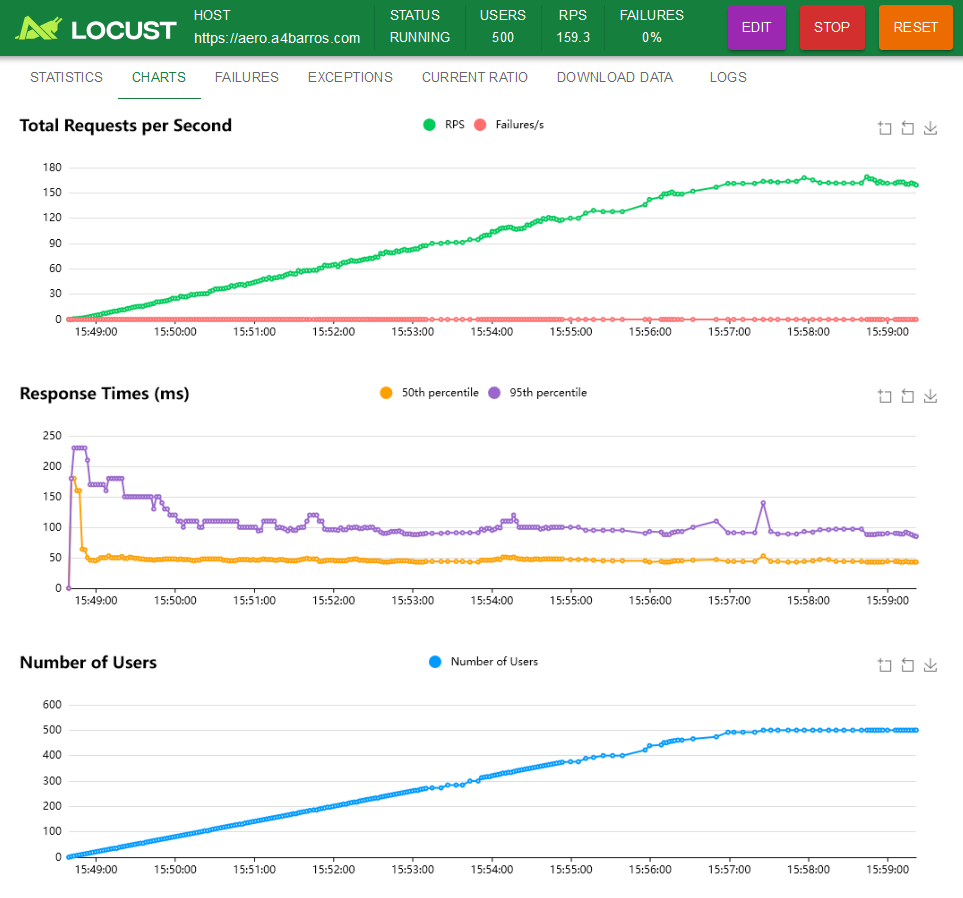
\includegraphics[width=0.6\linewidth]{img/locust-cache.png}
    \end{center}
\end{frame}


\section{Conclusão}
\begin{frame}{Demonstração}
    \begin{center}
        \url{https://aero.a4barros.com}
    \end{center}
\end{frame}

\begin{frame}{Obrigado}
    \centering
    \Huge Obrigado! \\
    \normalsize Perguntas?
\end{frame}

\end{document}

